\chapter{Kiến thức liên quan}
\label{chap:related_work}
% -------------------------------------------------------------------
% Introduction of the chapter
% -------------------------------------------------------------------
Để phát triển giải pháp ứng dụng công nghệ theo dõi chuyển động mắt hỗ trợ trẻ rối loạn đọc, chúng ta cần nắm vững kiến thức về rối loạn đọc, các bất thường trong chuyển động mắt của trẻ, cũng như những kiến thức liên quan đến việc ứng dụng công nghệ theo dõi mắt để hỗ trợ nhóm trẻ này. Trong \textbf{Chương 2}, khóa luận sẽ trình bày tổng quan các kiến thức về rối loạn đọc, cũng như những công nghệ liên quan được sử dụng để hoàn thành khóa luận. 
% -------------------------------------------------------------------
% Dyslexia and abnormalities in eye movements
% -------------------------------------------------------------------
\section{Rối loạn đọc và sự khác thường trong chuyển động mắt của người mắc chứng rối loạn đọc}
\label{sec:dysevm}
Rối loạn đọc (Dyslexia) là một hội chứng rối loạn học tập ảnh hưởng đến khả năng đọc chính xác và lưu loát của một cá nhân, được đặc trưng bởi các khó khăn trong nhận diện từ, giải mã từ và đánh vần \cite{roitsch2019overview, american2013diagnostic}. Những người mắc rối loạn đọc thường gặp trở ngại trong việc ánh xạ âm thanh trong ngôn ngữ nói sang ký tự viết, đặc biệt ở các ngôn ngữ có mối quan hệ phức tạp giữa chữ cái và âm thanh chúng biểu thị. Rối loạn đọc không chỉ gây khó khăn trong học tập mà còn có thể dẫn đến các vấn đề tâm lý và xã hội, chẳng hạn như cảm giác thất vọng, tự ti hoặc bị cô lập. Mặc dù có trí thông minh bình thường, trẻ mắc rối loạn đọc thường không đạt được kỹ năng đọc ngang bằng với bạn bè đồng trang lứa, dẫn đến việc bị hiểu lầm là lười biếng hoặc kém thông minh. Hơn nữa, đây là một trong những rối loạn học tập phổ biến nhất, ảnh hưởng từ 5-10\% dân số toàn cầu \cite{khaleghi2022developing}. Do đó, việc chẩn đoán và can thiệp kịp thời cho người mắc rối loạn đọc là rất quan trọng.

Các phương pháp hiện tại để chẩn đoán rối loạn đọc bao gồm kiểm tra kỹ năng đọc, đánh giá ngữ âm, kiểm tra tâm lý, và phỏng vấn phụ huynh cùng giáo viên \cite{lindstrom2019dyslexia}. Tuy nhiên, rối loạn đọc không phải là một căn bệnh mà là một rối loạn phát triển, với biểu hiện khác nhau ở mỗi cá nhân \cite{al2012understanding}. Vì vậy, việc áp dụng cùng một phương pháp chẩn đoán và can thiệp cho tất cả các cá nhân mắc cùng một rối loạn có thể không phản ánh được khó khăn cụ thể của từng người, cũng như không thể đề xuất các biện pháp cá nhân hóa. Bên cạnh các phương pháp đánh giá truyền thống, những cách tiếp cận cho phép quan sát trực tiếp hành vi và chuyển động mắt của từng cá nhân đang ngày càng nhận được sự quan tâm. Nhờ sự phát triển công nghệ, các bài kiểm tra đánh giá đã được số hóa và tích hợp với công nghệ theo dõi chuyển động mắt, mang đến những khả năng mới trong việc chẩn đoán khách quan và chính xác. Phần lớn các nghiên cứu đều cho thấy rằng trẻ rối loạn đọc thường có những đặc điểm chuyển động mắt khác thường so với những trẻ phát triển bình thường khác cùng trang lứa. Nghiên cứu của Jainta và cộng sự tiết lộ rằng người mắc rối loạn đọc kém hơn trong việc kiểm soát song nhãn cầu \cite{jainta2011dyslexic}. Suy giảm thị giác-vận động nhãn cầu ở những người này có thể gây mất ổn định điểm cố định, dẫn đến ảnh hưởng khả năng đọc hiểu. Ngoài ra, trẻ mắc rối loạn đọc thiếu hụt trong quá trình xử lý thông tin, không chỉ đối với văn bản \cite{jones2008elucidating, weiss2022lateralization} mà còn với các kích thích khác như hình ảnh khuôn mặt \cite{galazka2021facial, aasberg2022left}. Sự thiếu hụt này biểu hiện qua dao động liên tục và chuyển động mắt tương đối nhỏ ở trẻ mắc rối loạn đọc so với trẻ phát triển bình thường khi đọc. Đồng thời, trẻ rối loạn đọc cũng có tần suất chuyển động tiến và lùi của nhãn cầu cao hơn đáng kể \cite{pavlidis1985eye}. Những bất thường trong chuyển động mắt này cho thấy tiềm năng lớn của việc ứng dụng công nghệ theo dõi chuyển động mắt để hỗ trợ chẩn đoán và can thiệp rối loạn đọc.


% -------------------------------------------------------------------
% Eye-tracking technology
% -------------------------------------------------------------------
\section{Kiến thức nền tảng}
\label{sec:theoreticalbg}
Bên cạnh những hiểu biết về chứng rối loạn đọc và các bất thường trong chuyển động mắt của người mắc hội chứng này, các kiến thức liên quan đến công nghệ theo dõi chuyển động mắt, nhận diện khu vực quan tâm, nhận dạng ký tự quang học, các đặc trưng chuyển động mắt có giá trị trong việc hỗ trợ trẻ rối loạn đọc, cũng như các phương pháp trực quan hóa, đều đóng vai trò quan trọng trong quá trình ứng dụng công nghệ này để hỗ trợ nhóm đối tượng trên. Trong phần tiếp theo, chúng tôi sẽ trình bày tổng quan những kiến thức có liên quan.

\subsection{Công nghệ theo dõi chuyển động mắt}
\label{subsec:et}
Công nghệ theo dõi chuyển động mắt (Eye tracking) là một phương pháp thu thập và nhận diện chuyển động của mắt khi con người nhìn từ vị trí này sang vị trí khác \cite{poole2006eye}. Theo dõi chuyển động mắt đo lường vị trí và thời điểm ánh mắt hướng tới khi thực hiện một nhiệm vụ hoặc hành động. Công nghệ này xác định mối liên hệ giữa mắt và hệ thần kinh, liên kết chuyển động của mắt với quá trình nhận thức và từ đó đưa ra một cái nhìn sâu rộng vào hoạt động bên trong của não bộ \cite{carter2020best}. 

\begin{figure}[h]
    \centering
    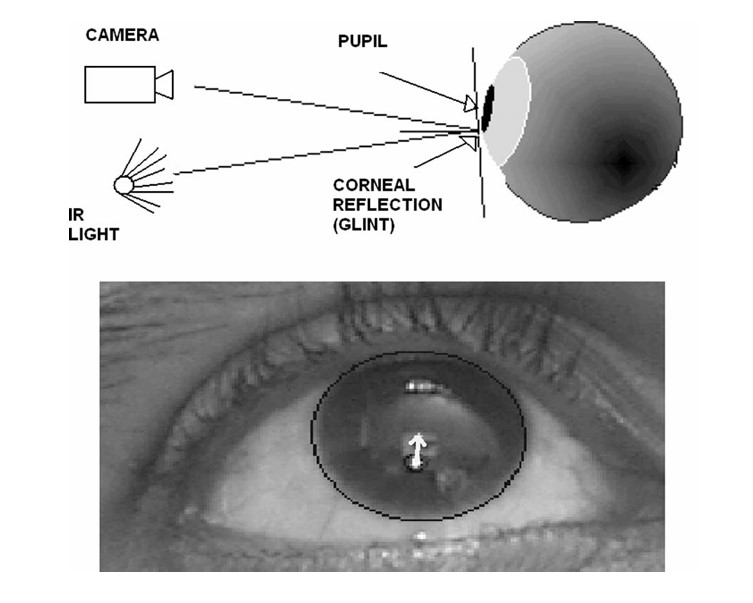
\includegraphics[width=0.8\columnwidth]{Chapter2/pccr.jpg}
    \caption{Sơ đồ biểu diễn kỹ thuật PCCR (ở trên) và vectơ ước tính từ tâm mống mắt đến điểm phản xạ \cite{sigut2010iris}}
    \label{fig:pccr}
\end{figure}

Trong những năm gần đây, theo dõi chuyển động mắt nhận được sự chú ý mạnh mẽ từ cộng đồng nghiên cứu. Những công bố từ các lĩnh vực khác nhau như tâm lý, giáo dục đặc biệt, v.v. đều sử dụng theo dõi chuyển động mắt như một công cụ đáng tin cậy cho việc khám phá những câu hỏi có liên quan đến việc phân bố sự chú ý trực quan. Chuyển động mắt được theo dõi và ghi nhận thông qua máy theo dõi chuyển động mắt (eye tracker). Trong số các kỹ thuật được áp dụng để theo dõi và ghi nhận chuyển động mắt, phương pháp Trung tâm đồng tử phản xạ giác mạc (Pupil Center Corneal Reflection - PCCR) là kỹ thuật phổ biến nhất và được tích hợp rộng rãi trong các thiết bị theo dõi chuyển động mắt hiện đại \cite{punde2017study, sigut2010iris}. Hình \ref{fig:pccr} minh họa một mô hình thiết lập điển hình của phương pháp PCCR. Góc của trục thị giác được xác định dựa trên vị trí tương đối giữa tâm đồng tử và điểm phản xạ trên giác mạc, với giả định rằng điểm phản xạ trên giác mạc sẽ không thay đổi khi vị trí của camera và nguồn sáng là cố định. Do đó, khi mắt xoay làm thay đổi vị trí của tâm đồng tử, góc tạo bởi tâm đồng tử và điểm phản xạ giác mạc cũng thay đổi tương ứng, từ đó cho phép tính toán chuyển động của mắt. Bên cạnh đó, nhiều thiết bị theo dõi chuyển động mắt hiện đại sử dụng nguồn sáng hồng ngoại nhằm tăng độ chính xác trong việc phát hiện tâm đồng tử, đồng thời giảm thiểu ảnh hưởng từ các yếu tố gây nhiễu như kính điều chỉnh tật khúc xạ hoặc ánh sáng môi trường.

% -------------------------------------------------------------------
% Area of Interest
% -------------------------------------------------------------------
\subsection{Nhận diện khu vực quan tâm}
\label{subsec:aoi}
Trong các nghiên cứu ứng dụng công nghệ theo dõi chuyển động mắt, thuật ngữ "khu vực quan tâm" (Areas of Interest – AOI) là một khái niệm phổ biến và đóng vai trò quan trọng. Khu vực quan tâm đề cập đến những vùng xác định, có thể có hình dạng bất kỳ, bao quanh các đối tượng cụ thể trong kích thích thị giác mà người quan sát tập trung ánh nhìn vào \cite{lagmay2022enhanced}. Việc phân tích chuyển động mắt trên toàn bộ kích thích thường tốn nhiều công sức và khó làm nổi bật được các đặc trưng liên quan đến từng yếu tố trong kích thích thị giác. Do đó, việc tập trung phân tích theo khu vực quan tâm giúp cung cấp các thước đo cục bộ, hỗ trợ hiệu quả hơn cho các nghiên cứu về sự chú ý và mức độ tập trung \cite{hessels2016area}. Các chỉ số định lượng từ khu vực quan tâm, chẳng hạn như thời gian nhìn chăm chú (dwell time), góp phần làm cho dữ liệu chuyển động mắt dễ phân tích và diễn giải hơn, đồng thời được ứng dụng rộng rãi trong nhiều lĩnh vực nghiên cứu như tương tác người–máy và tâm lý học \cite{hessels2016area}. Lý tưởng nhất là mỗi khu vực quan tâm nên có đường viền trùng khớp với hình dạng thực tế của đối tượng được quan sát, tuy nhiên, do một số đối tượng có hình dạng hoặc kích thước phức tạp và khó xác định chính xác, các khu vực quan tâm trong thực tế thường được biểu diễn bằng các hình học đơn giản như hình chữ nhật, hình elip, v.v. \cite{mahanama2022eye}.

Trong các nghiên cứu liên quan đến hội chứng rối loạn đọc, khu vực quan tâm thường được xác định tại các vùng chứa văn bản, chẳng hạn như toàn bộ đoạn văn (được xác định là vùng văn bản mở rộng khoảng 0.5 cm xung quanh) \cite{bonifacci2023eye}, các câu đơn lẻ trong văn bản \cite{bonifacci2023eye, raatikainen2021detection}, hoặc các từ riêng lẻ \cite{luniewska2022effect}. Bên cạnh đó, khu vực quan tâm cũng được áp dụng trong một số nghiên cứu về khả năng xử lý khuôn mặt ở trẻ mắc chứng rối loạn đọc, với dữ liệu đầu vào là hình ảnh hoặc video \cite{galazka2021facial, aasberg2022left}.


% -------------------------------------------------------------------
% Optical character recognition
% -------------------------------------------------------------------
\subsection{Nhận diện ký tự quang học}
\label{subsec:ocr}
Như đã trình bày trong mục \ref{subsec:aoi}, trong các bài toán ứng dụng công nghệ theo dõi chuyển động mắt nhằm hỗ trợ người mắc chứng rối loạn đọc, các khu vực quan tâm thường được xác định tại những vùng chứa văn bản. Trong những năm gần đây, nhờ sự phát triển mạnh mẽ của các kỹ thuật thị giác máy tính, việc xác định các khu vực quan tâm một cách tự động đã trở nên ngày càng dễ dàng. Đối với các khu vực liên quan đến văn bản, các thuật toán nhận dạng ký tự quang học (Optical Character Recognition – OCR) thường được sử dụng. Nhận dạng ký tự quang học là quá trình chuyển đổi hình ảnh điện tử của văn bản viết tay, đánh máy hoặc in ấn thành dạng văn bản mà máy tính có thể xử lý và hiểu được \cite{singh2012survey}. Phương pháp nhận dạng ký tự quang học cho phép tự động trích xuất thông tin từ văn bản và nhập vào cơ sở dữ liệu điện tử, thay thế cho việc nhập liệu thủ công. Công nghệ này đã được ứng dụng rộng rãi trong nhiều lĩnh vực như pháp luật (số hóa tài liệu pháp lý), ngân hàng (xử lý séc tự động), và chăm sóc sức khỏe (trích xuất thông tin từ biểu mẫu bệnh nhân), giúp tăng hiệu quả xử lý dữ liệu và giảm thiểu thời gian cũng như công sức.

\begin{figure}[h]
    \centering
    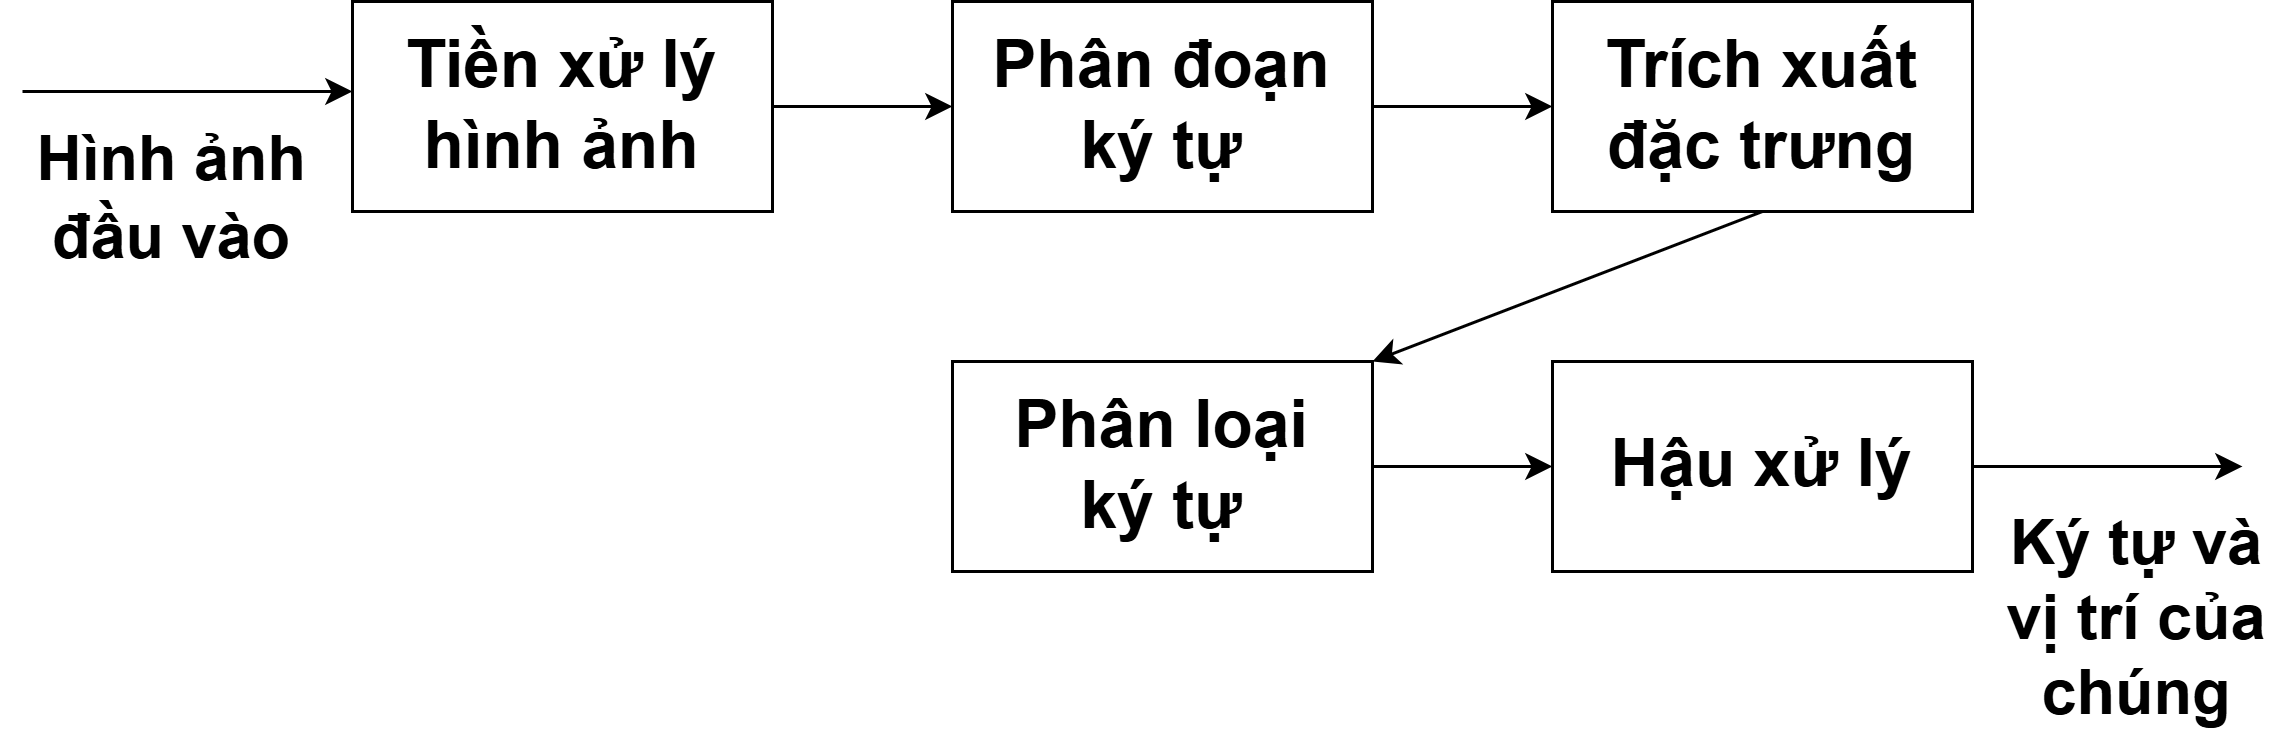
\includegraphics[width=0.8\columnwidth]{Chapter2/ocr.png}
    \caption{Tổng quan quy trình của thuật toán nhận dạng ký tự quang học}
    \label{fig:ocr}
\end{figure}

Có nhiều phương pháp nhận dạng ký tự quang học với các cách tiếp cận khác nhau, tuy nhiên, phần lớn các thuật toán đều tuân theo một quy trình gồm các bước cơ bản sau: thu thập hình ảnh, tiền xử lý, phân đoạn ký tự, trích xuất đặc trưng, phân loại ký tự và hậu xử lý \cite{islam2017survey}. Quá trình này được minh họa trong Hình \ref{fig:ocr}. Đầu tiên, hình ảnh văn bản được thu thập từ các nguồn khác nhau như văn bản in hoặc viết tay. Ở bước tiền xử lý, các kỹ thuật như chỉnh thẳng, phân tích bố cục hoặc phân ngưỡng được sử dụng để xử lý và làm sạch hình ảnh nguồn ở mức tổng thể, giúp văn bản dễ nhận diện hơn và giảm thiểu hoặc loại bỏ nhiễu. Sau đó, các ký tự được phân đoạn để tách riêng và chuẩn bị cho bước nhận dạng bằng các kỹ thuật như phân tích thành phần kết nối và hình chiếu. Tại bước trích xuất đặc trưng, hệ thống xác định các đặc điểm có khả năng phân biệt giữa các ký tự. Các đặc trưng này sau đó được đưa vào bộ phân loại để nhận dạng ký tự tương ứng dựa trên các kỹ thuật như phân loại cấu trúc, phân loại mẫu, v.v. Cuối cùng, bước hậu xử lý được áp dụng nhằm tinh chỉnh và nâng cao độ chính xác của kết quả nhận dạng. 




\subsection{Các đặc trưng của chuyển động mắt}
\label{subsec:emvm}

Trong các bài toán liên quan đến chuyển động mắt, việc tìm hiểu và lựa chọn các đặc trưng chuyển động mắt phù hợp là yếu tố hết sức quan trọng. Vì vậy, trong nội dung tiếp theo, khóa luận sẽ trình bày các hiểu biết liên quan đến những đặc trưng chuyển động mắt thường được sử dụng trong các nghiên cứu ứng dụng công nghệ theo dõi chuyển động mắt nhằm hỗ trợ người mắc chứng rối loạn đọc, bao gồm điểm nhìn, điểm dừng, đường trượt và hồi quy.

\begin{figure}[h]
    \centering
    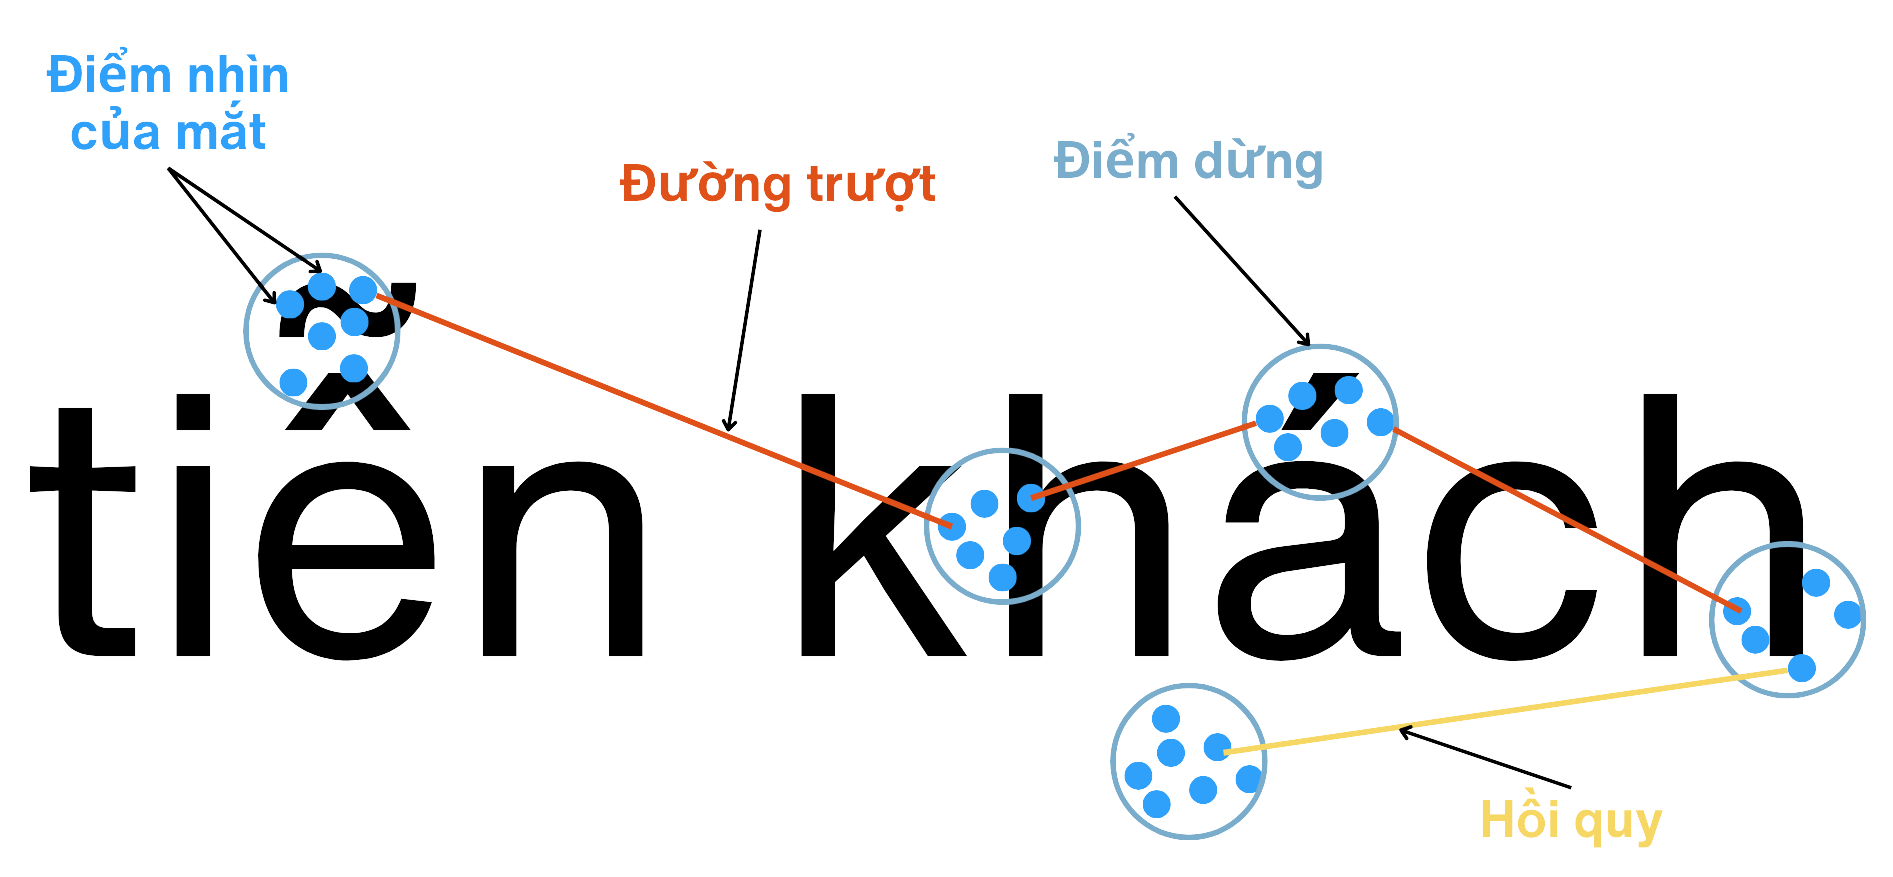
\includegraphics[width=0.9\columnwidth]{Chapter2/features.png}
    \caption{Các đặc trưng của chuyển động mắt: điểm nhìn của mắt, điểm dừng, đường trượt và hồi quy}
    \label{fig:features}
\end{figure}

\subsubsection{Điểm nhìn của mắt (Eye-gaze)}
Trong các nghiên cứu ứng dụng công nghệ theo dõi chuyển động mắt, phần lớn các thiết bị ghi nhận chuyển động mắt đều thu thập dữ liệu dưới dạng các điểm nhìn, biểu thị bởi các tọa độ \(x - y\) trên màn hình kèm theo thông tin thời gian tương ứng với từng điểm nhìn. Số lượng điểm nhìn thu được tỷ lệ thuận với khoảng thời gian người tham gia quan sát màn hình. Tuy nhiên, trong nhiều trường hợp, dữ liệu điểm nhìn có thể gây ra những khó khăn nhất định cho các nhà nghiên cứu do mật độ điểm quá lớn, dẫn đến khó khăn trong việc phân tích và phát hiện các đặc điểm đáng chú ý. Do đó, tùy vào mục tiêu cụ thể và phương pháp tiếp cận của từng nghiên cứu, dữ liệu điểm nhìn có thể được sử dụng trực tiếp hoặc được xử lý để trích xuất các đặc trưng trung gian giúp việc quan sát và phân tích trở nên hiệu quả hơn. Một số đặc trưng phổ biến thường được sử dụng bao gồm: điểm dừng, đường trượt và hồi quy, được minh họa trong Hình \ref{fig:features}.


\subsubsection{Điểm dừng (Fixation)}
\label{subsubsec:fix}
Điểm dừng là đặc trưng mà mắt của con người nhìn cố định vào một mục tiêu thị giác cụ thể, đồng thời duy trì sự ổn định trong nhận thức và tiếp nhận thông tin thị giác của mắt \cite{rayner200935th}. Quá trình tính toán điểm dừng giúp đơn giản hóa đáng kể dữ liệu chuyển động mắt bằng cách hợp nhất các điểm riêng lẻ thành một điểm dữ liệu hợp nhất \cite{salvucci2000identifying}. Vì vậy, việc sử dụng điểm dừng góp phần đơn giản hóa tập dữ liệu, đồng thời vẫn bảo toàn các đặc trưng cốt lõi có giá trị trong phân tích và nghiên cứu.

Nhiều đặc trưng thống kê của điểm dừng được sử dụng trong phân tích chuyển động mắt, tùy thuộc vào từng vấn đề cụ thể, bao gồm số lượng điểm dừng, thời lượng điểm dừng, vị trí của điểm dừng tại mỗi từ, v.v, mỗi chỉ số phản ánh các khía cạnh khác nhau của hành vi thị giác \cite{poole2006eye}. Chẳng hạn, số lượng điểm dừng và thời lượng của mỗi điểm dừng phản ánh quá trình nhận thức và xử lý ngôn ngữ ở thời gian thực. Số lượng điểm dừng ít và thời lượng điểm dừng ngắn cho thấy quá trình xử lý song song diễn ra tốt, vì trong khi đọc, việc xử lý văn bản và định hướng chuyển động mắt diễn ra đồng thời \cite{poole2006eye}. Trong nhiều thí nghiệm, trẻ rối loạn đọc thường cho thấy các đặc trưng thống kê điểm dừng khác biệt, chẳng hạn như thời lượng điểm dừng dài hơn và số lượng điểm dừng nhiều hơn so với trẻ phát triển bình thường. Những quan sát này cho thấy rằng nhóm trẻ này cần nhiều thời gian hơn để phân tích, thu thập thông tin, nhận thức và xử lý từ vựng \cite{parshina2022global},  cũng như khả năng phối hợp chuyển động mắt kém hiệu quả hơn \cite{kirkby2008binocular}.


\subsubsection{Đường trượt (Saccade)}
\label{subsubsec:sac}
Đường trượt là đặc trưng về chuyển động nhanh của mắt di chuyển từ một điểm dừng này đến điểm dừng tiếp theo \cite{carter2020best}. Nhiều nghiên cứu đã chỉ ra rằng sự điều khiển tốt hệ thống đặc trưng chuyển động của mắt, trong đó có đường trượt và điểm dừng, là rất cần thiết cho việc đọc \cite{levy1979control}. Khi ta nhận biết hình ảnh, chúng ta sẽ thu thập thông tin tại mỗi điểm dừng và chuyển vùng lấy thông tin thông qua đường trượt. Đường trượt được ghi lại có thể phản ánh khoảng cách và mối liên hệ theo trật tự thời gian của tiến trình xử lý thông tin trong quá trình định danh hình ảnh \cite{roitsch2019overview}. 

Trẻ rối loạn đọc thường có số đường trượt nhiều hơn và độ dài của mỗi đường trượt ngắn hơn khi so sánh với những trẻ phát triển bình thường. Nguyên nhân của việc thực hiện nhiều đường trượt là do sự hạn chế về mặt nhạy bén trong quá trình xử lý thông tin thị giác \cite{seassau2014binocular}. Ngoài ra, độ dài của đường trượt lớn còn cho thấy khả năng đọc trôi chảy và tự tin, trong khi đó đường trượt nhỏ biểu thị khả năng đọc khó khăn \cite{smyrnakis2021silent}.


\subsubsection{Hồi quy (Regression)}
\label{subsubsec:reg}
Hồi quy, hay còn gọi là chuyển động giật lùi của mắt (regressive saccade), là một đặc trưng thị giác đại diện cho chuyển động của mắt theo hướng ngược lại với tiến trình đọc hoặc quan sát. Đối với người đọc bình thường, hồi quy thường xuất hiện tại điểm dừng cuối cùng của một dòng văn bản và hướng về các điểm dừng nằm ở phía bên trái của các vị trí đó \cite{booth2013function}.

Sự xuất hiện của các chuyển động hồi quy có thể bắt nguồn từ nhiều nguyên nhân khác nhau. Trước hết, trong quá trình đọc, mắt có thể bỏ qua những từ mang thông tin quan trọng hoặc rời khỏi điểm dừng trước khi quá trình xử lý thông tin thị giác hoàn tất, dẫn đến sự không chắc chắn trong việc tiếp nhận nội dung \cite{inhoff2019regressions}. Hiện tượng này thường được quan sát thấy rõ hơn khi người đọc xử lý các văn bản có cấu trúc phức tạp, chứa lỗi ngữ pháp hoặc mang nội dung mơ hồ, những yếu tố làm gia tăng mức độ không chắc chắn về mặt thông tin \cite{inhoff2009word}. Bên cạnh đó, hồi quy còn liên hệ chặt chẽ với năng lực trí nhớ công việc (working memory), khi nó đóng vai trò như một cơ chế hỗ trợ người đọc hồi tưởng lại những thông tin đã đọc trước đó, đặc biệt trong trường hợp các văn bản dài và đòi hỏi khả năng lưu giữ và tích hợp thông tin cao \cite{spivey2013thinking}. Trong các nghiên cứu về rối loạn đọc, người mắc chứng này thường có tần suất hồi quy cao hơn đáng kể so với người đọc bình thường, phản ánh quá trình xử lý, tiếp nhận và hiểu văn bản kém hiệu quả hơn, cũng như những hạn chế về trí nhớ công việc.


\subsection{Các phương pháp trực quan hoá}
\label{subsec:visual}
Các đặc trưng của chuyển động mắt được trình bày tại Mục \ref{subsec:emvm} thường là các đặc trưng mang tính thống kê. Để trực quan hóa những đặc trưng này, các phương pháp như bản đồ nhiệt và đường quét thường được sử dụng trong các bài toán ứng dụng công nghệ theo dõi chuyển động mắt để hỗ trợ người mắc chứng rối loạn đọc. Trong nội dung tiếp theo, khóa luận sẽ trình bày tổng quan về hai phương pháp trực quan hóa phổ biến này. 
\subsubsection{Bản đồ nhiệt (Heatmap)}
\label{subsubsec:heatmap}

Một trong những phương pháp trực quan hóa dữ liệu được ứng dụng rộng rãi trong các nghiên cứu sử dụng công nghệ theo dõi chuyển động mắt là bản đồ nhiệt. Bản đồ nhiệt phản ánh phân bố không gian của chuyển động mắt trên các kích thích thị giác, mà không bao hàm yếu tố thời gian, từ đó cung cấp cái nhìn tổng quan về hành vi quan sát của người tham gia. Trong bối cảnh nghiên cứu chứng rối loạn đọc, bản đồ nhiệt đặc biệt hữu ích trong việc xác định những vùng mà trẻ tập trung ánh nhìn nhiều hơn (hoặc ít hơn) trên ngữ liệu kích thích, qua đó cho phép đánh giá mức độ chú ý hoặc những khu vực đòi hỏi nhiều nỗ lực nhận diện và xử lý ngôn ngữ hơn từ phía trẻ \cite{mahanama2022eye}. Trong thực tiễn, bản đồ nhiệt thường được biểu diễn dưới dạng Mô hình Hỗn hợp Gaussian (Gaussian Mixture Model - GMM), nhằm mô tả xác suất hoặc tần suất xuất hiện của các điểm dừng mắt. Việc sử dụng GMM trong trực quan hóa dữ liệu sẽ được trình bày chi tiết tại Mục \ref{subsec:visualizee}. Kết quả của quá trình này được hiển thị thông qua một mặt nạ mã hóa màu được chồng lên hình ảnh kích thích thị giác mà người tham gia quan sát. Các vùng có màu “nóng” (chẳng hạn như đỏ, cam hoặc vàng) biểu thị sự tập trung cao hơn, trong khi các màu “lạnh” (như xanh lá cây) phản ánh mức độ chú ý thấp hơn \cite{mahanama2022eye}.

Thông thường, bản đồ nhiệt chủ yếu được ứng dụng trong các nghiên cứu liên quan đến hành vi quan sát trên các giao diện người dùng, chẳng hạn như trang web hoặc công cụ tìm kiếm thông tin, trong khi việc sử dụng bản đồ nhiệt trong các nghiên cứu về hỗ trợ trẻ mắc chứng rối loạn đọc, đặc biệt với ngôn ngữ tiếng Anh, vẫn còn hạn chế. Tuy nhiên, do sự khác biệt đáng kể giữa tiếng Việt và tiếng Anh đã được trình bày trong phần Đặt vấn đề, nghiên cứu này khai thác bản đồ nhiệt như một công cụ trực quan để phân tích hành vi quan sát của trẻ, nhằm xác định các vần trong một từ mà trẻ tập trung nhìn vào nhiều hơn hoặc mất nhiều thời gian hơn để xử lý.

\begin{figure}[h]
    \centering
    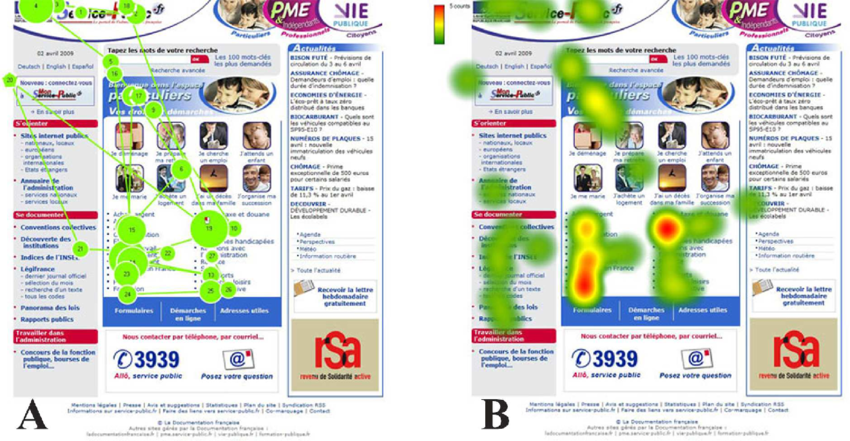
\includegraphics[width=\columnwidth]{Chapter2/heatmap-scanpath.png}
    \caption{Hình ảnh đường quét (trái) và bản đồ nhiệt (phải) thể hiện dữ liệu chuyển động mắt của người dùng trên một trang web \cite{drusch2014analysing}}
    \label{fig:heatmap-scanpath}
\end{figure}

\subsubsection{Đường quét (Scan path)}
\label{subsubsec:scanpath}
Đường quét thể hiện mô hình chuyển động của mắt trong một nhiệm vụ thị giác, phản ánh cả hai chiều không gian và thời gian thông qua chuỗi các điểm dừng và đường trượt. Khác với bản đồ nhiệt chỉ cung cấp tổng quan về mật độ quan sát, đường quét cho phép phân tích chi tiết hơn về hành vi nhìn, bao gồm các vị trí mà người tham gia tập trung sự chú ý, thứ tự quan sát, mức độ chú ý tại từng khu vực, cũng như chiến lược di chuyển ánh nhìn trên kích thích thị giác \cite{mahanama2022eye}. Thông thường, đường quét được biểu diễn dưới dạng chuỗi các nút (đại diện cho vị trí điểm dừng) và các cạnh kết nối (đại diện cho đường trượt giữa các điểm dừng liên tiếp), được phủ trực tiếp lên ngữ liệu thị giác, với đường kính của mỗi nút thường tỉ lệ thuận với thời gian cố định tại vị trí đó \cite{goldberg2010scanpath}. Phân tích đường quét đã được ứng dụng rộng rãi trong nhiều lĩnh vực như sinh trắc học, khoa học thần kinh, và đặc biệt là trong các nghiên cứu về rối loạn đọc. Al-Wabil và cộng sự \cite{al2008examining} chỉ ra rằng những người mắc chứng rối loạn đọc có xu hướng có các đường quét không ổn định hơn, cũng như ít mang tính chiến lược hơn khi tương tác với các cấu trúc điều hướng trên giao diện web. Ngoài ra, nghiên cứu của Parshina và cộng sự \cite{appadurai2022image} cũng cho thấy mặc dù có những đặc điểm chung trong các đường quét giữa các cá nhân, vẫn tồn tại sự khác biệt đáng kể phản ánh phong cách đọc riêng biệt của từng người. Từ đó, đường quét được xem là một công cụ giàu tiềm năng để phân tích sự khác biệt giữa các cá nhân hoặc nhóm đối tượng thông qua dữ liệu chuyển động mắt. Ví dụ về đường quét và bản đồ nhiệt được thể hiện ở Hình \ref{fig:heatmap-scanpath}.

% -------------------------------------------------------------------
% Chapter summary
% -------------------------------------------------------------------
\section{Kết chương}
Chương này đã trình bày các hiểu biết về rối loạn đọc, cũng như những kiến thức nền tảng về công nghệ được sử dụng để phát triển giải pháp trong khóa luận, bao gồm công nghệ theo dõi chuyển động mắt, khu vực quan tâm, thuật toán nhận diện ký tự quang học, các đặc trưng của chuyển động mắt, cũng như các phương pháp trực quan hoá. 
